% Capítulo 4: decisões encadeadas (else if) para a situação do aluno.
\documentclass[border=4pt]{standalone}
\usepackage[utf8]{inputenc}
\usepackage[T1]{fontenc}
% Estilo comum dos fluxogramas e diagramas de blocos.
\usepackage{tikz}
\usetikzlibrary{arrows.meta, positioning, calc, shapes.geometric, shapes.misc}
\definecolor{navy}{RGB}{23,45,80}
\definecolor{laranja}{RGB}{250,110,29}
\definecolor{cinzalogo}{RGB}{107,114,126}
\definecolor{azul}{RGB}{205,222,247}
\tikzset{
  base/.style={draw=navy, line width=0.9pt, font=\sffamily\small, align=center, inner sep=4pt},
  terminal/.style={base, rounded rectangle, fill=laranja!45, draw=laranja, minimum width=20mm, minimum height=7mm},
  processo/.style={base, rectangle, fill=laranja!12, minimum width=28mm, minimum height=8mm},
  decisao/.style={base, diamond, aspect=2.2, fill=azul, inner sep=1pt, minimum width=30mm},
  es/.style={base, trapezium, trapezium left angle=72, trapezium right angle=108,
             fill=white, minimum width=26mm, minimum height=8mm, trapezium stretches body},
  fluxo/.style={-{Stealth[length=2.2mm]}, navy, line width=0.9pt},
  rotulo/.style={font=\sffamily\small\bfseries, text=navy},
  legenda/.style={font=\sffamily\scriptsize, text=cinzalogo},
  resposta/.style={font=\sffamily\scriptsize\bfseries, text=navy},
}

\begin{document}
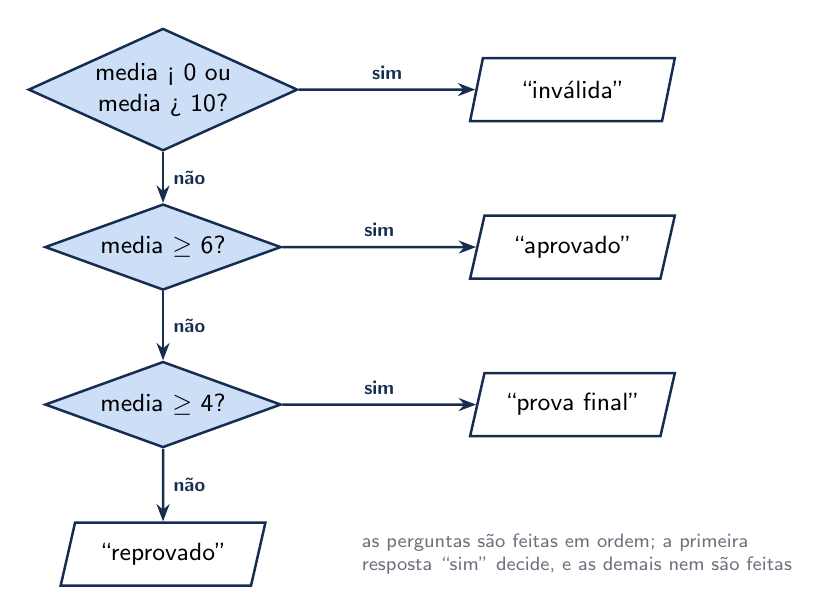
\begin{tikzpicture}
  \node[decisao] (d1) at (0, 0) {media < 0 ou\\media > 10?};
  \node[decisao] (d2) at (0, -2.0) {media $\geq$ 6?};
  \node[decisao] (d3) at (0, -4.0) {media $\geq$ 4?};
  \node[es] (s1) at (5.2, 0) {``inválida''};
  \node[es] (s2) at (5.2, -2.0) {``aprovado''};
  \node[es] (s3) at (5.2, -4.0) {``prova final''};
  \node[es] (s4) at (0, -5.9) {``reprovado''};
  \draw[fluxo] (d1) -- node[resposta, above] {sim} (s1);
  \draw[fluxo] (d2) -- node[resposta, above] {sim} (s2);
  \draw[fluxo] (d3) -- node[resposta, above] {sim} (s3);
  \draw[fluxo] (d1) -- node[resposta, right] {não} (d2);
  \draw[fluxo] (d2) -- node[resposta, right] {não} (d3);
  \draw[fluxo] (d3) -- node[resposta, right] {não} (s4);
  \node[legenda, align=left, anchor=west] at (2.4, -5.9)
    {as perguntas são feitas em ordem; a primeira\\resposta ``sim'' decide, e as demais nem são feitas};
\end{tikzpicture}
\end{document}
